
\documentclass[12pt, a4paper]{book}

%% Übersetzen als Entwurf
%\usepackage[entwurf]{bhtThesis}
%% Übersetzen für die Abgabe
\usepackage[abgabe]{bhtThesis}
\let\ifpdf\relax	%bhtThesis nutzt \ifpdf

\usepackage{blindtext}   %für Blindtext in Kapitel 2

\usepackage{listings}             % Include the listings-package
\renewcommand\lstlistlistingname{Quelltextverzeichnis}	%Übersetzung
\renewcommand{\lstlistingname}{Quelltext}	%Übersetzung

\newcommand*\ttvar[1]{\texttt{\expandafter\dottvar\detokenize{#1}\relax}}
\newcommand*\dottvar[1]{\ifx\relax#1\else
	\expandafter\ifx\string_#1\string_\allowbreak\else#1\fi
	\expandafter\dottvar\fi}

\usepackage{xcolor}
\usepackage{xparse}% to define star variant of macro
\makeatletter
\def\lst@MSkipToFirst{%
	\global\advance\lst@lineno\@ne
	\ifnum \lst@lineno=\lst@firstline
	\def\lst@next{\lst@LeaveMode \global\lst@newlines\z@
		\lst@OnceAtEOL \global\let\lst@OnceAtEOL\@empty
		\ifnum \c@lstnumber>0
		\vspace{2 mm}
		\fi
		\lst@InitLstNumber % Added to work with modified \lsthk@PreInit.
		\lsthk@InitVarsBOL
		\c@lstnumber=\numexpr-1+\lst@lineno % this enforces the displayed line numbers to always be the input line numbers
		\lst@BOLGobble}%
	\expandafter\lst@next
	\fi}
\makeatother

\lstset{ 
  literate={ö}{{\"o}}1
           {ä}{{\"a}}1
           {ü}{{\"u}}1
           {Ö}{{\"O}}1
           {Ä}{{\"A}}1
           {Ü}{{\"U}}1
           {ß}{{\ss}}1,
%  language=C,
  numbers=left,
  stepnumber=1,
  tabsize=2,
  breaklines=true,
  basicstyle=\ttfamily\footnotesize,
  columns=fullflexible,
  frame=single,
  alsoother={_-},
%  breakatwhitespace=false,
  alsoletter={()[]=},
  postbreak=\mbox{\textcolor{red}{$\hookrightarrow$}},
  keepspaces=true
}

\usepackage{multirow}
\usepackage{array}
\newcolumntype{L}[1]{>{\raggedright\let\newline\\\arraybackslash\hspace{0pt}}m{#1}}
\newcolumntype{C}[1]{>{\centering\let\newline\\\arraybackslash\hspace{0pt}}m{#1}}
\newcolumntype{R}[1]{>{\raggedleft\let\newline\\\arraybackslash\hspace{0pt}}m{#1}}

\usepackage[breaklinks=true]{hyperref}

\usepackage{textcomp}

\usepackage{wrapfig}	%wrapfigure

\renewcommand{\textdownarrow}{$\downarrow$}
\renewcommand{\textleftarrow}{$\leftarrow$}

\usepackage{pdfpages}	%includepdf
\usepackage{grffile}	%spaces in filenames
\usepackage{chngcntr}	%continous footnote numbering (no reset from chapter to chapter)
\counterwithout{footnote}{chapter}	%setting for package chngcntr
\usepackage[n, operators, logic]{cryptocode}	%for crypto, pseudocode and protocol flow graphs
\usepackage{placeins}	%for \FloatBarrier
%\usepackage{float}		%for H option for floats
\usepackage{caption}	%captionof in minipage und source (siehe unten)

\newcommand{\source}[1]{\vspace{-10pt}\caption*{{#1}}}

\usepackage{xargs}                      % Use more than one optional parameter in a new commands
\definecolor{OliveGreen}{cmyk}{0.64,0,0.95,0.40}
\definecolor{Plum(traditional)}{rgb}{0.56, 0.27, 0.52}
\usepackage[colorinlistoftodos,prependcaption,textsize=tiny]{todonotes}
\newcommandx{\unsure}[2][1=]{\todo[linecolor=red,backgroundcolor=red!25,bordercolor=red,#1]{#2}}
\newcommandx{\change}[2][1=]{\todo[linecolor=blue,backgroundcolor=blue!25,bordercolor=blue,#1]{#2}}
\newcommandx{\info}[2][1=]{\todo[linecolor=OliveGreen,backgroundcolor=OliveGreen!25,bordercolor=OliveGreen,#1]{#2}}
\newcommandx{\improvement}[2][1=]{\todo[linecolor=Plum(traditional),backgroundcolor=Plum(traditional)!25,bordercolor=Plum(traditional),#1]{#2}}
\newcommandx{\thiswillnotshow}[2][1=]{\todo[disable,#1]{#2}}

\usepackage{microtype}	%better typesetting
\usepackage[nopostdot, acronyms, nonumberlist, style=altlist, toc]{glossaries} %glossary, option: no location within the glossary %section=chapter, 
%\usepackage{glossaries-extra} %print all unused glossary entries
\makeglossaries
\loadglsentries{glossary}
\glsaddall


\hyphenation{Schlüs-sel-aus-tausch hash-en-den} %Worttennungen

\usepackage[]{appendix}

\usepackage{dirtree} %directory tree

\usepackage[bottom]{footmisc} %figures not below footnotes

%Bibliographie:
\usepackage[numbers, round]{natbib}
\bibliographystyle{alphadin}

%Flowcharts
\usepackage{tikz}
\usetikzlibrary{shapes.geometric, arrows}

\tikzstyle{startstop} = [rectangle, rounded corners, minimum width=3cm, minimum height=1cm,text centered, draw=black, fill=red!30]
\tikzstyle{io} = [trapezium, trapezium left angle=70, trapezium right angle=110, minimum width=3cm, minimum height=1cm, text centered, text width=3cm, draw=black, fill=blue!30]
\tikzstyle{process} = [rectangle, minimum width=3cm, minimum height=1cm, text centered, text width=3cm, draw=black, fill=orange!30]
\tikzstyle{decision} = [diamond, minimum width=3cm, minimum height=1cm, text centered, text width=3cm, draw=black, fill=green!30]
\tikzstyle{arrow} = [thick,->,>=stealth]
%Flowcharts end


%%
%% Es folgen einige Zusätze, die in Kapitel 1 beschriben sind. 
%% Alles was nicht notwendig ist, kann auskommentiert werden
%%
\usepackage{trsym}
\usepackage{bytefield}
\usepackage{lstlangarm}

%%
%% Use git metadata
%%
\usepackage[missing={gitHeadInfo.gin not found!}]{gitinfo2}

%%
%% Pfad zu den Bildern
%%
\graphicspath{
  {pictures/}
}

%%
%% Persönliche macros 
%%


%% Message
\typeout{---------------------------------------------------------------}
\typeout{----> document.tex ---- Zentrales Dokument---------------------}
\typeout{---------------------------------------------------------------}

%TODO: add gitinfo
\version{}
\datum{\today}
%%
%% Titel, Autor und Betreuer
%%
\fachbereich{VI -- Informatik und Medien --} 
\studiengang{Technische Informatik - Embedded Systems}
\autor{Kayoko Abe, Oleksandra Baga, Heiko Radde}
\edvnr{826058, 849852, 887027}
\titel{Dynamische Flüssigkeitssimulation auf einem RGB-Würfel}

%%\renewcommand{\baselinestretch}{1.05} 
\begin{document}
\pagestyle{fancy}
%\pagenumbering{empty}

%%
%% Beuth Hochschule für Technik --  Abschlussarbeit
%%
%% Titelseiten und Erklärungen 
%%
%%%%%%%%%%%%%%%%%%%%%%%%%%%%%%%%%%%%%%%%%%%%%%%%%%%%%%%%%%%%%%%%%%%%%

\pagenumbering{roman}
\maketitle
\clearpage
%\thispagestyle{empty}
% Rueckseite (leer)
%% 
~
%\newpage
%
%\section*{Kurzfassung}
%Die Kurzfassung gibt ein kurzes und prägnantes Bild der gesamten Arbeit. Sie soll den Leser neugierig machen und klarmachen, was zu erwarten ist. Erreichte Ergebnisse werden kurz umrissen.



%\clearpage
%
%\section*{Erklärung}
%Ich  versichere, dass ich diese Abschlussarbeit ohne fremde Hilfe selbstständig verfasst und nur die angegebenen Quellen und Hilfsmittel benutzt habe. Wörtlich oder dem Sinn nach aus anderen Werken entnommene Stellen sind unter Angabe der Quellen kenntlich gemacht.
%\vspace{10ex}\\
%
%\hrule
%{\small{14.08.2018}}\hfill{\small{Unterschrift}}

\microtypesetup{protrusion=false}
\tableofcontents
\listoffigures
\lstlistoflistings
\cleardoublepage
\pagenumbering{arabic}
\microtypesetup{protrusion=true}
%\listoftodos[Notes]


%%%%%%%%%%%%%%%%%%%%%%%%%%%%%%%%%%%%%%%%%%%%%%%%%%%%%%%%%%%%%%%
%% Die Kapitel der Arbeit

%\todo{Todo}
%\unsure{unsure}
%\change{change}
%\info{info}
%\improvement{improvement}

\pagenumbering{arabic}

\clearpage
\chapter{Einführung}
\label{chap:einfuehrung}
%verbale Formulierung der Aufgabenstellung, erste Abschätzung der Aufwände
Im Rahmen des Moduls `Fortgeschrittene ARM Programmierung' wird der Keil Evaluation Board MCB2388 verwenden, welcher einen NXP LPC2388 Microcontroller installiert und verschiedene Schnittstellen wie LCD, USB oder Ethernet besitzt. Der ARM7-Prozessor auf dem Board kann mit der bis zu seinesr höchsten Betriebsfrequenz von ?? MHz getaktet werden. Diese Merkmale lassen unterschiedliche Applikationen umsetzen.

Insbesondere unter Berücksichtigung von seiner hohen Taktrate sind wir zur Idee gekommen, Flüssigkeit zu simulieren und in 3 Dimension anhand eines aus 6 LED-Matrix Panels aufgebauten Würfel zu visualisieren. Zur Realisierung unseres Projekts sollte eine sehr hohe Taktrate benötigt werden, um die Bewegung der Wasserteilchen auszurechnen und diese auf den LED Panels in Echtzeit zu übertragen. Zusätzlich zu dem Entwicklungsboard sowie zu den Panels wird ein Accelerometer benötigt, um die 3-D Position des Würfels zu bestimmen und die Flüssigkeit darin entsprechend zu visualisieren.

Im folgenden Kapital wird die detaillierte Beschreibung jeder Komponente bezüglich der Theorie und der Implementierung vorgestellt.

%Main oscillator = 1M - 24 MHz
%Max cpu operating takt with PLL = 
%output from multiplier OCC = 275M - 550 MHz



\chapter{Implementierung}
\label{chap:implementierung}
%Einleitung zur Implementierung
%Sprache, Stiel, Debugging, IDE, etc.
\section{Entwicklungsumgebung}
Zur Entwicklung der Softwarekomponente soll erst Keil\textsuperscript{\scriptsize\textregistered} Microcontroller Development Kit (MDK) auf einem Rechner installiert werden. Das Kit ist besonders gut geeignet für Arm\textsuperscript{\scriptsize\textregistered}-basierte Microcontroller und beinhaltet alle notwendigen Komponente für Embedded Applikationen. Die Edition MDK-Lite ist konstenlos jedoch mit der Beschränkung von 32KBytes Codegröße verfügbar. Zusätzlich muss Legacy Package ARMv7 (NXP LPC 2388) installiert werden. Anschließend soll die Integrierte Entwicklungsumgebung Keil $\mu$version 5 erfolgreich installiert sein.

Der Board kann durch einen USB-Anschluss vom Rechner eingeschaltet werden. Der ULINK-ME kann ebenfalls durch einen USB-Anschluss zum Laden des Programms und zum Debuggen verwendet werden.
Die Software für den RaspberryPi 1B wurde mit den \texttt{arm-none-eabi gcc}, basierend auf \texttt{GCC 4.5.2} von CodeSourcery kompilliert.

Sämtlicher Quellcode des Projekts wurde in C geschrieben und Doxygen-konform dokumentiert.

%Beschreibung der Konfiguration von IDE

\section{Pinbelegung}
Der Accelerometer und ein der 6 Panels werden durch freie GPIO-Pins mit dem Board verbunden. Abbildung \ref{fig:pins} zeigt diese Pinbelegung. Es ist dabei zu beachten, die bereits vom Hersteller belegten Pins zu vermeiden, um den Board erfolgreich in Betrieb zu nehmen.

Die belegten Pins und die relevanten Ports 2 und 3 müssen wie Code \ref{code:led-init} initialisiert werden, um diese als GPIO/Output-Pins verwenden zu können.

\begin{figure}
	\centering
	\includegraphics[width=0.8\linewidth]{example-image}
	\caption[Pinbelegung]{Pinbelegung}
	\label{fig:pins}
\end{figure}

\newpage
\clearpage
\label{chap:impl:sph}
%Beschreibung der Implementierung der SPH-Flüssigkeitssimulation

\section{Partikel-basierte Simulation}
Es gibt zwei grundlegende Ansätze für die Simulation von Flüssigkeiten: entweder auf Gittern oder auf Partikeln basierend. Die Repräsentation von Simulationen in einem Gitter ist genauer, jedoch ebenso rechenintensiver \cite{fluid.tutorial_paper}. Da dieses Projekt auf Mikrocontrollern umgesetzt und die Flüssigkeit auf einem Bildschirm mit niedriger Auflösung angezeigt werden soll fiel die Wahl auf die Partikel-basierte Simulation.

\subsection{Grundlagen}

Die Simulation von Flüssigkeiten beruht auf den Navier Stokes Gleichungen \cite{fluid.tutorial_paper}\footnote{$\overrightarrow{u}$ ist die Geschwindigkeit der Flüssigkeit, $\rho$ die Dichte. Der Druck innerhalb der Flüssigkeit wird durch $p$ dargestellt und $v$ entspricht der kinematische Viskosität}: 

\begin{align}
	\frac{\partial \overrightarrow{u}}{\partial t} + \overrightarrow{u} + \frac{1}{\rho} \nabla p &= \overrightarrow{F} + v \nabla \cdot \nabla \overrightarrow{u} \\
	\nabla \cdot \overrightarrow{u} &= 0
\end{align}

\cite{fluid.website} und \cite{fluid.website2} führt aus, wie mit Hilfe der Kernel \texttt{poly6}, \texttt{spiky} und \texttt{viscosity} die folgenden Formeln für die Dichte, den Druck und die Viskosität erstellt werden können:

\begin{align}
	\rho_i &= \sum^{j} m_j W(|r_i - r_j|, h) \\
	F_i^{pressure} &= - \sum^{j} m_i m_j (\frac{p_i}{\rho_j^2} + \frac{p_j}{\rho_j^2}) \nabla W(|r_i - r_j|, h) \\
	F_i^{viscosity} &= \eta \sum^{j} m_j \frac{|u_j - u_i|}{\rho_j} \nabla^2 W(|r_i - r_j|, h)
\end{align}

Für die einzelnen Kernel gilt:
\begin{align}
	W_{poly6}(r, h) &= \frac{315}{56 \pi h^9} 	\begin{cases}
													(h^2 - r^2)^3,   & 0 \leq r \leq h\\
													0, & \text{andernfalls}\\
												\end{cases} \\
	W_{spiky}(r, h) &= \frac{15}{\pi h^6}		\begin{cases}
													(h - r),   & 0 \leq r \leq h\\
													0, & \text{andernfalls}\\
												\end{cases} \\
	W_{viscosity}(r, h) &= \frac{15}{2 \pi h^3}		\begin{cases}
													-\frac{r^3}{2h^3} + \frac{r^2}{h^2} + \frac{h}{2r} - 1,   & 0 \leq r \leq h\\
													0, & \text{andernfalls}\\
												\end{cases}
\end{align}

Ein Problem in der Simulation ist, dass alle Partikel auf alle anderen einwirken. Dies stellt eine $O(n^2)$ Beziehung da, die sich sehr negativ auf den Rechenaufwand auswirkt. Ein Weg die Berechnung zu Beschleunigen beruht auf dem Fakt, dass der Einfluss von entfernteren Partikeln auf das gerade betrachtete stetig abnimmt. Wenn man nun die aktuelle Position der Partikel auf einem Schachbrett aufträgt, so reicht es nur die Partikel, die sich in den umliegenden Feldern befinden, in die Berechnung der Kräfte die auf einen gegebenen Partikel wirken, zu betrachten.

\subsection{Umsetzung}

Die Simulation der Partikel wurde in \texttt{C} für den 2D-Raum umgesetzt. In einem 2D-Array sind in jedem Eintrag doppelt verkettete Listen aus den Partikeln verlinkt, die sich aktuell innerhalb dem Feld befinden (siehe \ref{code.sph.structs}). Zur Berechnung der nächsten Position eines jeden Partikels werden Dichte, Druck und Viskosität des Partikels unter Berücksichtigung der Umliegenden berechnet. Addiert man nun die soeben berechneten Kräfte mit der extern Einwirkenden (Erdanziehungskraft) und integriert dies über die verstrichene Zeit erhält man den Beschleunigungsvektor des Teilchens. Die Multiplikation der Beschleunigung mit der verstrichenen Zeit ergibt nun die Positionsveränderung des Partikels.

\begin{lstlisting}[language={c}, caption={Datenstrukturen der SPH}, label={code.sph.structs}]
typedef struct
{
	double position[2];
	double velocity[2];
	double mass;
	double density;
	double pressure;
	double force[2];
} particle_t;


typedef struct particle_list_element_s
{
	particle_t particle;
	struct particle_list_element_s* prev;
	struct particle_list_element_s* next;
} particle_list_element_t;


typedef struct
{
	particle_list_element_t* particle_list;
	uint32_t particle_count;
} particle_grid_element_t;

typedef particle_grid_element_t panel_t[PARTICLE_GRID_X][PARTICLE_GRID_Y];
\end{lstlisting}

\begin{wrapfigure}{r}{0.5\textwidth}
	\centering
	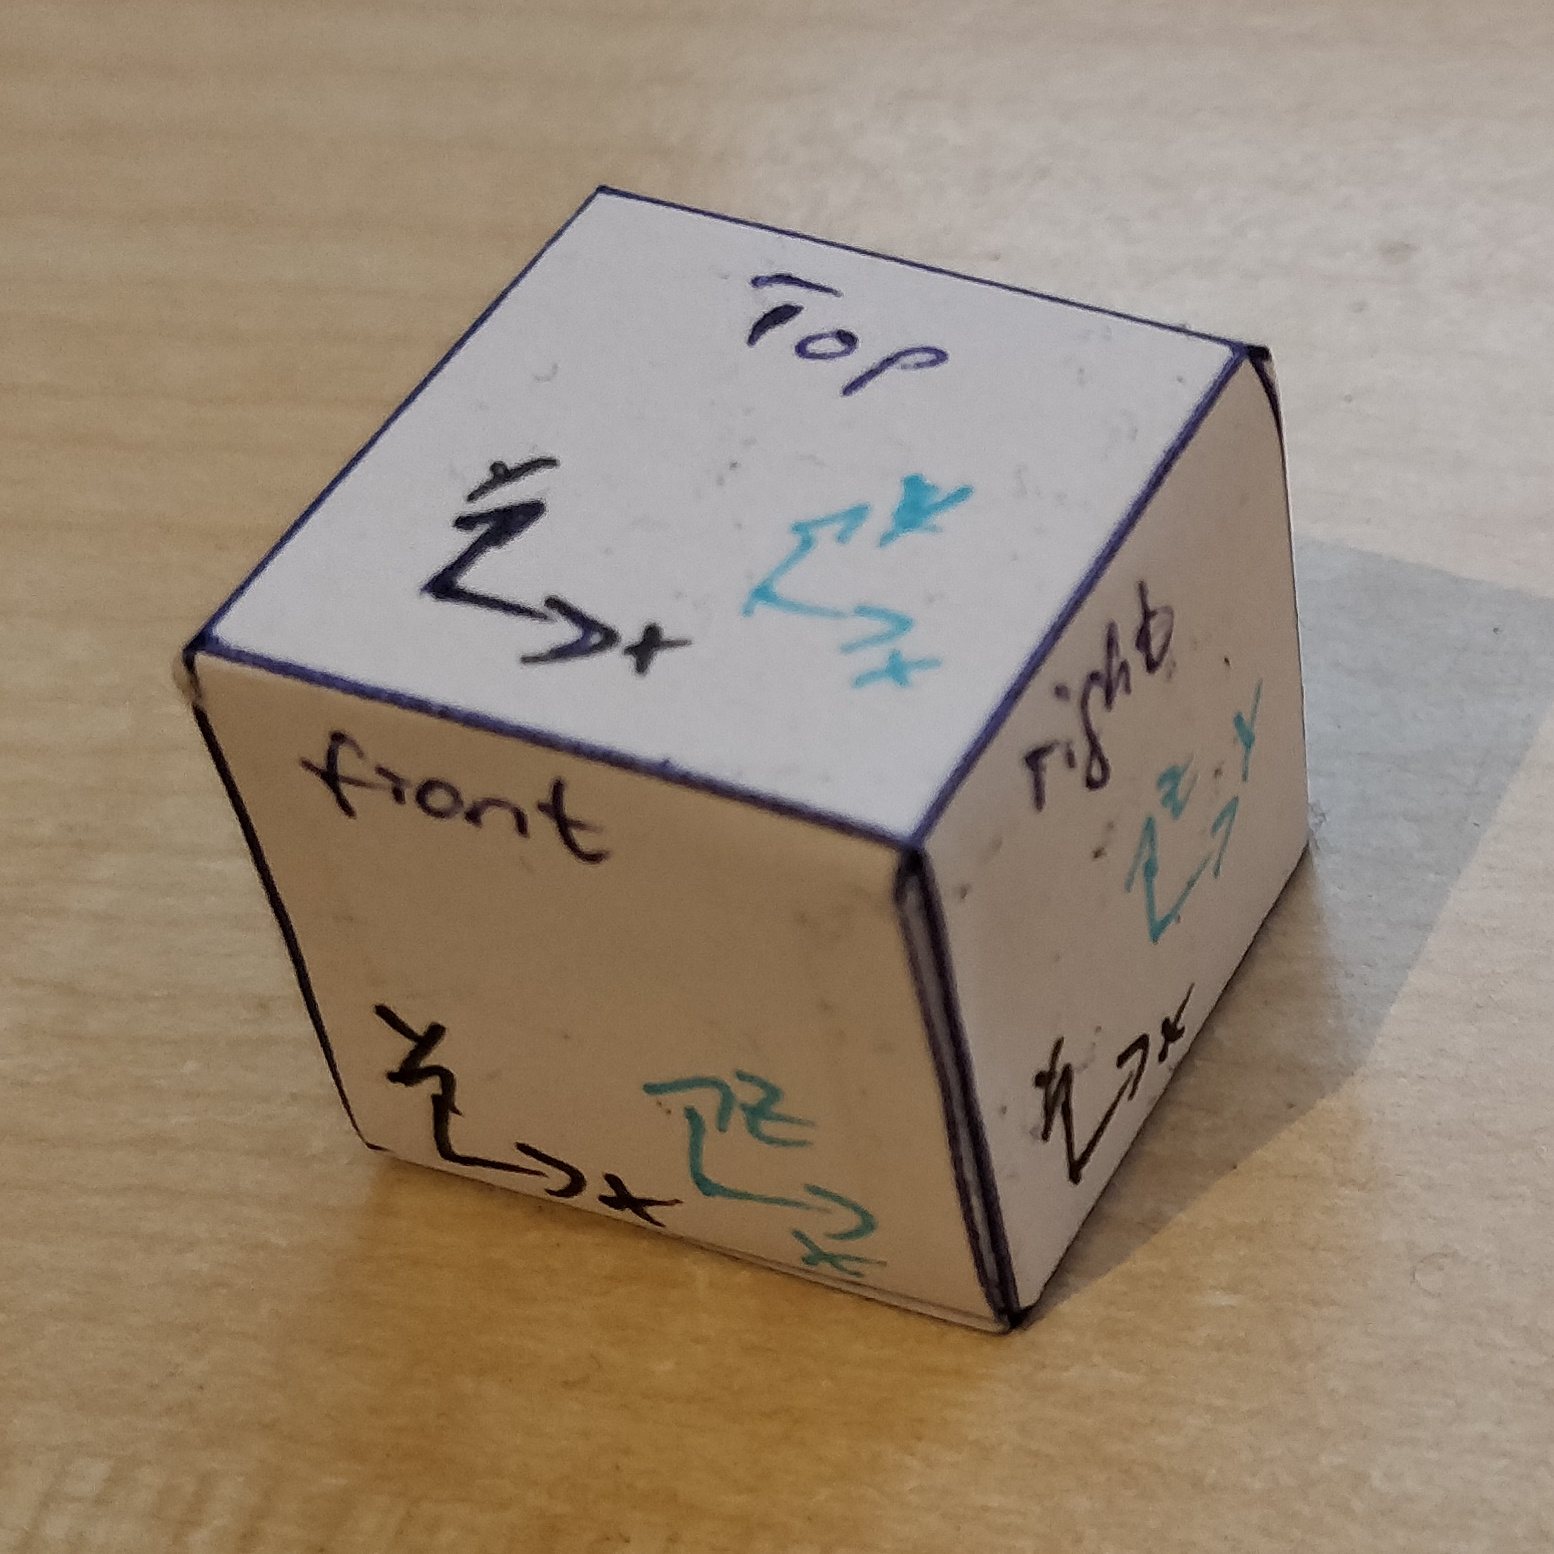
\includegraphics[width=.45\linewidth]{IMG_20190409_212603.jpg}
	\caption{Würfelmodell mit Koordinatensystem der LED-Panels und der 2D-Arrays}
	\label{fig:sph:cube_model}
\end{wrapfigure}

Um den Würfel darzustellen werden nun sechs der 2D-Arrays genutzt. Wenn die neue Position eines Partikels nun die Außengrenzen des Arrays überschreiten würde, so wird es auf die andere Würfelseite übertragen. Die Implementierung der Simulation wurde während der Entwicklung auf einem Linux-PC getestet. Hierzu wurde sie in ein Programm eingebettet, die Position der einzelnen Partikel ausließt und über X11 auf dem Bildschirm darstellt. Da die Simulation nur mit elementaren Rechenoperationen arbeitet konnte sie im Anschluss problemlos in das ARM-Programm eingefügt werden. Dieses stellt nun die Anzahl der Partikel in einem Feld der 2D-Arrays als Farbschattierung auf dem LED-Display dar.

\subsection{Rechenbeschleunigung durch RaspberryPi 1B}
\FloatBarrier

\begin{lstlisting}[caption={Memorymap des Raspberry Pi 1B}, label={code.sph.rp.memmap}]
MEMORY
{
	ram : ORIGIN = 0x8000, LENGTH = 0x1000
}

SECTIONS
{
	.text : { *(.text*) } > ram
	.bss  : { *(.bss* ) } > ram
}
\end{lstlisting}

\begin{lstlisting}[language={[ARM]{Assembler}}, caption={ARM ASM startup code}, label={code.sph.rp.startup}]
.globl _start
_start:
	ldr sp, stack_start
	ldr r0, thumb_start_add
	bx r0

stack_start: .word 0x8000
thumb_start_add: .word thumb_start
	.word 0
	.word 0

.thumb
.thumb_func
thumb_start:
	bl main
hang: b hang

\end{lstlisting}

\begin{figure}
	\begin{bytefield}[bitwidth=1.1em]{32}
		\bitheader{0-31} \\
		\wordbox{1}{sync-marker \tiny{\texttt{0xF3CFC3CF}}} \\
		\bitbox{8}{panel\_no} & \bitbox{8}{x\_position} & \bitbox{8}{y\_position} & \bitbox{8}{color} \\
		\bitbox[lrb]{24}{color}
	\end{bytefield}
	\caption{Raspberry Pi Pixeldaten}
	\label{fig:sph:rp:pixels}
\end{figure}

\begin{figure}
	\begin{bytefield}[bitwidth=1.1em]{32}
		\bitheader{0-31} \\
		\wordbox{1}{sync-marker \tiny{\texttt{0xF3CFC3CF}}} \\
		\wordbox{1}{force\_x \tiny{(double)}} \\
		\wordbox{1}{force\_y \tiny{(double)}} \\
		\wordbox{1}{force\_z \tiny{(double)}}
	\end{bytefield}
	\caption{MCB2388 Accelerometer Daten}
	\label{fig:sph:rp:acc_data}
\end{figure}

Mit der Zusammenführung aller Teilkomponenten (siehe auch die Kapitel \nameref{chap:impl:accel} und \nameref{chap:impl:ledcube}) wurde klar, dass die maximale Taktung des genutzten \texttt{LPC2388} zwar gerade so für eine flüssige Darstellung auf dem Würfel ausreicht, jedoch die Berechnungen der Simulation zu merklichen Stottern ($\geq 250$ms) führt. Auch das Triggern der Bildwiederholung via Timer-Interrupt führte zu keinem zufriedenstellendem Ergebnis: eine flüssige Darstellung war nur möglich, wenn der Intervall des Interrupts so weit hochgestellt wurde, dass er dauerhaft anliegt. Daraufhin entschieden wir uns die Simulation selber auf einen \texttt{Raspberry Pi 1B} auszulagern, da dieser mit einer Frequenz von 700MHz getaktet ist, etwa 10 mal höher als der \texttt{LPC2388}.

Der Pi ist, mit Hilfe von \cite{rp1.headless.github}, ohne Nutzung eines Betriebssystems programmiert worden. Auf ihm ist ein \texttt{BCM2835} als Prozessor mit integrierter GPU verbaut. Die GPU sicht auf der ersten Partition der FAT32 formatierten SD-Karte beim Startup nach den boot-dateien \texttt{bootcode.bin} und \texttt{start.elf} und ließt anschließend die \texttt{kernel.img} und lädt diese in den Speicher. Nun wird der reset des ARMs freigegeben, dieser führt dann die \texttt{kernel.img} aus. \texttt{bootcode.bin} und \texttt{start.elf} können ohne weiteres dem firmware-repository\footnote{Siehe \url{https://github.com/raspberrypi/firmware/tree/master/boot}, Zugriff am 10.04.2019} der raspberrypi foundation entnommen werden.

Der Programmcode wird mit dem \texttt{arm-none-eabi-gcc} kompilliert und gelinkt \footnote{Optionen: \texttt{-mfpu=vfp -march=armv6zk -mtune=arm1176jzf-s -nostdlib -nostartfiles -std=c99 -ffreestanding}}, die kernel.img wird aus der erstellten .elf mittels \texttt{arm-none-eabi-objcopy kernel.elf -O binary kernel.img} extrahiert. Hierbei ist es wichtig, beim Bauen der \texttt{.elf} eine Memorymap (Siehe \ref{code.sph.rp.memmap}) mit der Option \texttt{-T} mit einzubinden.

Die SPH Simulation wurde nun um eine Callback-option beim Wechsel eines Partikels zu einem anderen Feld erweitert. Diese löst eine Kommunikation mittels dem \texttt{UART0} aus (\cite{rp1.headless.github}[uartx01] und \cite{broadcom.bcm2835.user_manual}[S.177 ff]) die ein Update zu den betroffenen Pixeln zum \texttt{LPC2388} schickt (vgl. \ref{fig:sph:rp:pixels}). Letzterer überträgt in regelmäßigen Abständen die vom \texttt{ADXL345} (vgl. Kapitel \ref{chap:impl:accel}) ausgelesenen Werte an den Pi (vgl. \ref{fig:sph:rp:acc_data}). Das Empfangen dieser Bytes löst einen Interrupt aus, welcher diese parst und die Werte der externen Kräfte aktualisiert.

Die Schnittstelle \texttt{UART0} auf dem Board benötigt nur zwei Kabel \texttt{Tx} und \texttt{Rx}, welche mit den freien GPIO Pins auf Port 0.2 bzw. 0.3 verbunden werden. Der Softwareteil einschließlich einer Interrupt-Service-Routine sowie Senden und Empfangen der Daten hat sich größtenteils auf einen Referenz-Code bezogen und seine Beschreibung entfällt dementsprechend. Die Initialisierungsschritte insbesondere Einstellung einer gewünschten Baudrate wurden selbst angegangen und werden daher vorgelegt (Quelltext \ref{code:uart:init}).

\paragraph{Baudrate generieren} 
Mit Bezug auf \cite{nxp.lpc23xx.user_manual} (Kapitel 4.12.1) können die Werte für den relevanten Register zur Einstellung einer gewünschten Baudrate berechnet werden. Die Register lauten UART0 Divisor Latch (U0DLL, U0DLM) und UART0 Fractional Divider Register (DIVADDVAL, MULVAL). Die Berechnungsschritte werden hiernach unter Hinweis auf Abb. 83 von \cite{nxp.lpc23xx.user_manual} beschrieben.

%TODO check values in debug mode
\begin{enumerate}
\item $DL_{est} = PCLK/(16 \times BR) = 39,0625$, wobei $PCLK = 72 MHz$ und $BR = 115200$.
\item $DL_{est}$ ist keine ganze Zahl, dann $FR_{est} = 1,5$.
\item $DL_{est} = Int ( PCLK/(16 \times BR \times FR_{est}) ) = 26$.
\item $FR_{est} = PCLK/(16 \times BR \times DL_{est}) = 1,5024$.
\item $1,1 < FR_{est} < 1,9$, dann
\item $DivAddVal = table (FR_{est}) = 5$ und $MulVal = table (FR_{est}) = 8$.
\item $DLM = DL_{est}[15:8] =$ 0x00 und $DLL = DL_{est}[7:0] =$ 0x06.
\end{enumerate}

\begin{lstlisting}[language={c}, caption={Initialisierung von UART0. Der Funktionsparameter \texttt{baudrate} erwartet den Wert von 115200, worauf basierend die Werte von relevanten Register vorher berechnet wurden.}, label={code:uart:init}]
/**
 * @brief Initialize UART0 by the following steps:
 * 1. Power in PCONP register, set bit PCUART0 (default enabled)
 * 2. Peripheral clock in PCLK_SEL0 register, select PCLK_UART0
 * 3. Baud rate in U0LCR register, set bit DLAB = 1.
 * 4. UART Fifo: user bit fifo enable (bit 0) in register U0FCR to enable fifo.
 * 5. Pins, select UART pins and pin modes in register PINSEL and PINMODE
 * 6. Interrupts: set DLAB = 0 in register U0LCR. VICIntEnable register in VIC.
 *
 * @param[in] baudrate Baud rate of UART communication
 * @warn      Current init setting is for baud rate 115200, Osc 12 MHz, Sysclk 72 MHz.
*/
int uart0_init(unsigned long baudrate)
{
    PCONP |= PCUART0; ///< UART0 power/clock control

    if (115200 != baudrate)
    {
        // TODO baudrate generator algorithm for other variations if needed
        return 1;
    }

    /* Set 7:6 bit of PCLKSEL0
    * 00: PCLK = CCLK/4
    * 01: PCLK = CCLK
    * 10: PCLK = CCLK/2
    * 11: PCLK = CCLK/8
    */
    PCLKSEL0 |= 0x00; ///< PCLK_UART0

    U0LCR |= 0x83; ///< Enable access to Divisor Latches, 8 bits, 1 stop bit, no parity

    /*
    * UART0 Divisor Latch LSB register
    *
    * /f[
    *    UART0_baudrate = PCLK / [16 * (256 * U0DLM + U0DLL) * (1+ DivAddVal/MulVal)]
    * /f]
    *
    * See Fig 83. Algorithm for setting UART dividers in LPC23xx_um for details.
    */
    U0DLM = 0; // Higher 8 bits of Divisor
    U0DLL = 6; // Lower 8 bits of Divisor
    /* UART0 Fractional Divider Register controls prescaler for baud rate generator */
    // MULVAL = 8; DIVADDVAL = 5;
    U0FDR |= 0x05;
    U0FDR &= 0xFFFFFF0F;
    U0FDR |= 0x80;

    U0LCR &= 0x7F; ///< Disable access to Divisor Latches
    U0FCR |= 0x07; ///< Enable Rx and Tx FIFOs and clear them

    PINSEL0 |= 0x50; ///< Set Pins P0.2, P0.3 in TXD0, RXD0 mode (PMODE has to 00 (pull-up))

    if (0 == install_irq(UART0_INT, (void *)uart0_isr, HIGHEST_PRIORITY))
    {
        return 1;
    }
    
    U0IER |= (IER_RBR | IER_THRE | IER_RLS); ///< Enable three UART0 interrupt sources: RBR, THRE, Rx Line Status

    return 0;
}
\end{lstlisting}

\clearpage
\label{chap:impl:accel}
%Beschreibung der Implementierung der Kommunikation mit & Auswertung der Werte von dem Gyro

\section{Beschleunigungssensor}
\subsection{Hardware}
Für die Ermittlung der Ausrichtung des Würfels wurde ein digitaler Beschleunigungsmesser verwendet. Für das Projekt standen anfangs zwei Geräte zur Verfügung: BNO055 von Adafruit und ADXL345 von Analog Devices. Zwar ist der Beschleunigungsmesser von Adafruit mächtiger, da dieser mehr Messungen vornimmt und eine größere Genauigkeit ermöglicht, dennoch wurde das Projekt am Ende unter der Verwendung des Beschleunigungsmessers ADXL345 umgesetzt. Grund dafür war, dass nach mehreren Versuchen mit dem Gerät von Adafruit zu kommunizieren festgestellt wurde, dass der Beschleunigungsmesser nicht defekt war. In alle Registern des Bausteins anstatt der vorprogrammierte Daten liegt nur die Zahl \texttt{0xE5}, was laut dem Hersteller zeigt, dass die Registern beim Startup nicht geleert werden.

Für die Verwendung des ADXL345 sollte man in Programm nur die Adressen ändern und richtig alle Pins belegen. Die ALT ADDRESS wurde auf 1 gesetzt und die 7-Bit-I2C-Adresse für das Gerät wurde somit als \texttt{0x1D} festgelegt. In Programm wurde direkt die entsprechende 8-Bit-I2C-Adresse \texttt{0x3A} verwendet und die notwendige Änderung der Adresse in \texttt{0x3B} aus \texttt{0x3A} wurde gerade in I2C Routine erledigt. So kann man unterscheiden, ob es Lesen oder Schreiben Operation durchführen sollen werden. 

Es gibt keine internen Pull-Up- oder Pull-Down-Widerstände für nicht verwendete Pins. Daher gibt es keinen bekannten Status oder Standardstatus für den CS- oder ALT ADDRESS-Pin, wenn er potentialfrei bleibt oder nicht verbunden ist. Es ist erforderlich, dass der CS-Pin an VDD  angeschlossen ist und dass der ALT ADDRESS-Pin bei Verwendung von I2C entweder an VDD oder GND angeschlossen ist (wir haben an VDD angeschlossen).

\begin{figure}[!h]
	\centering
	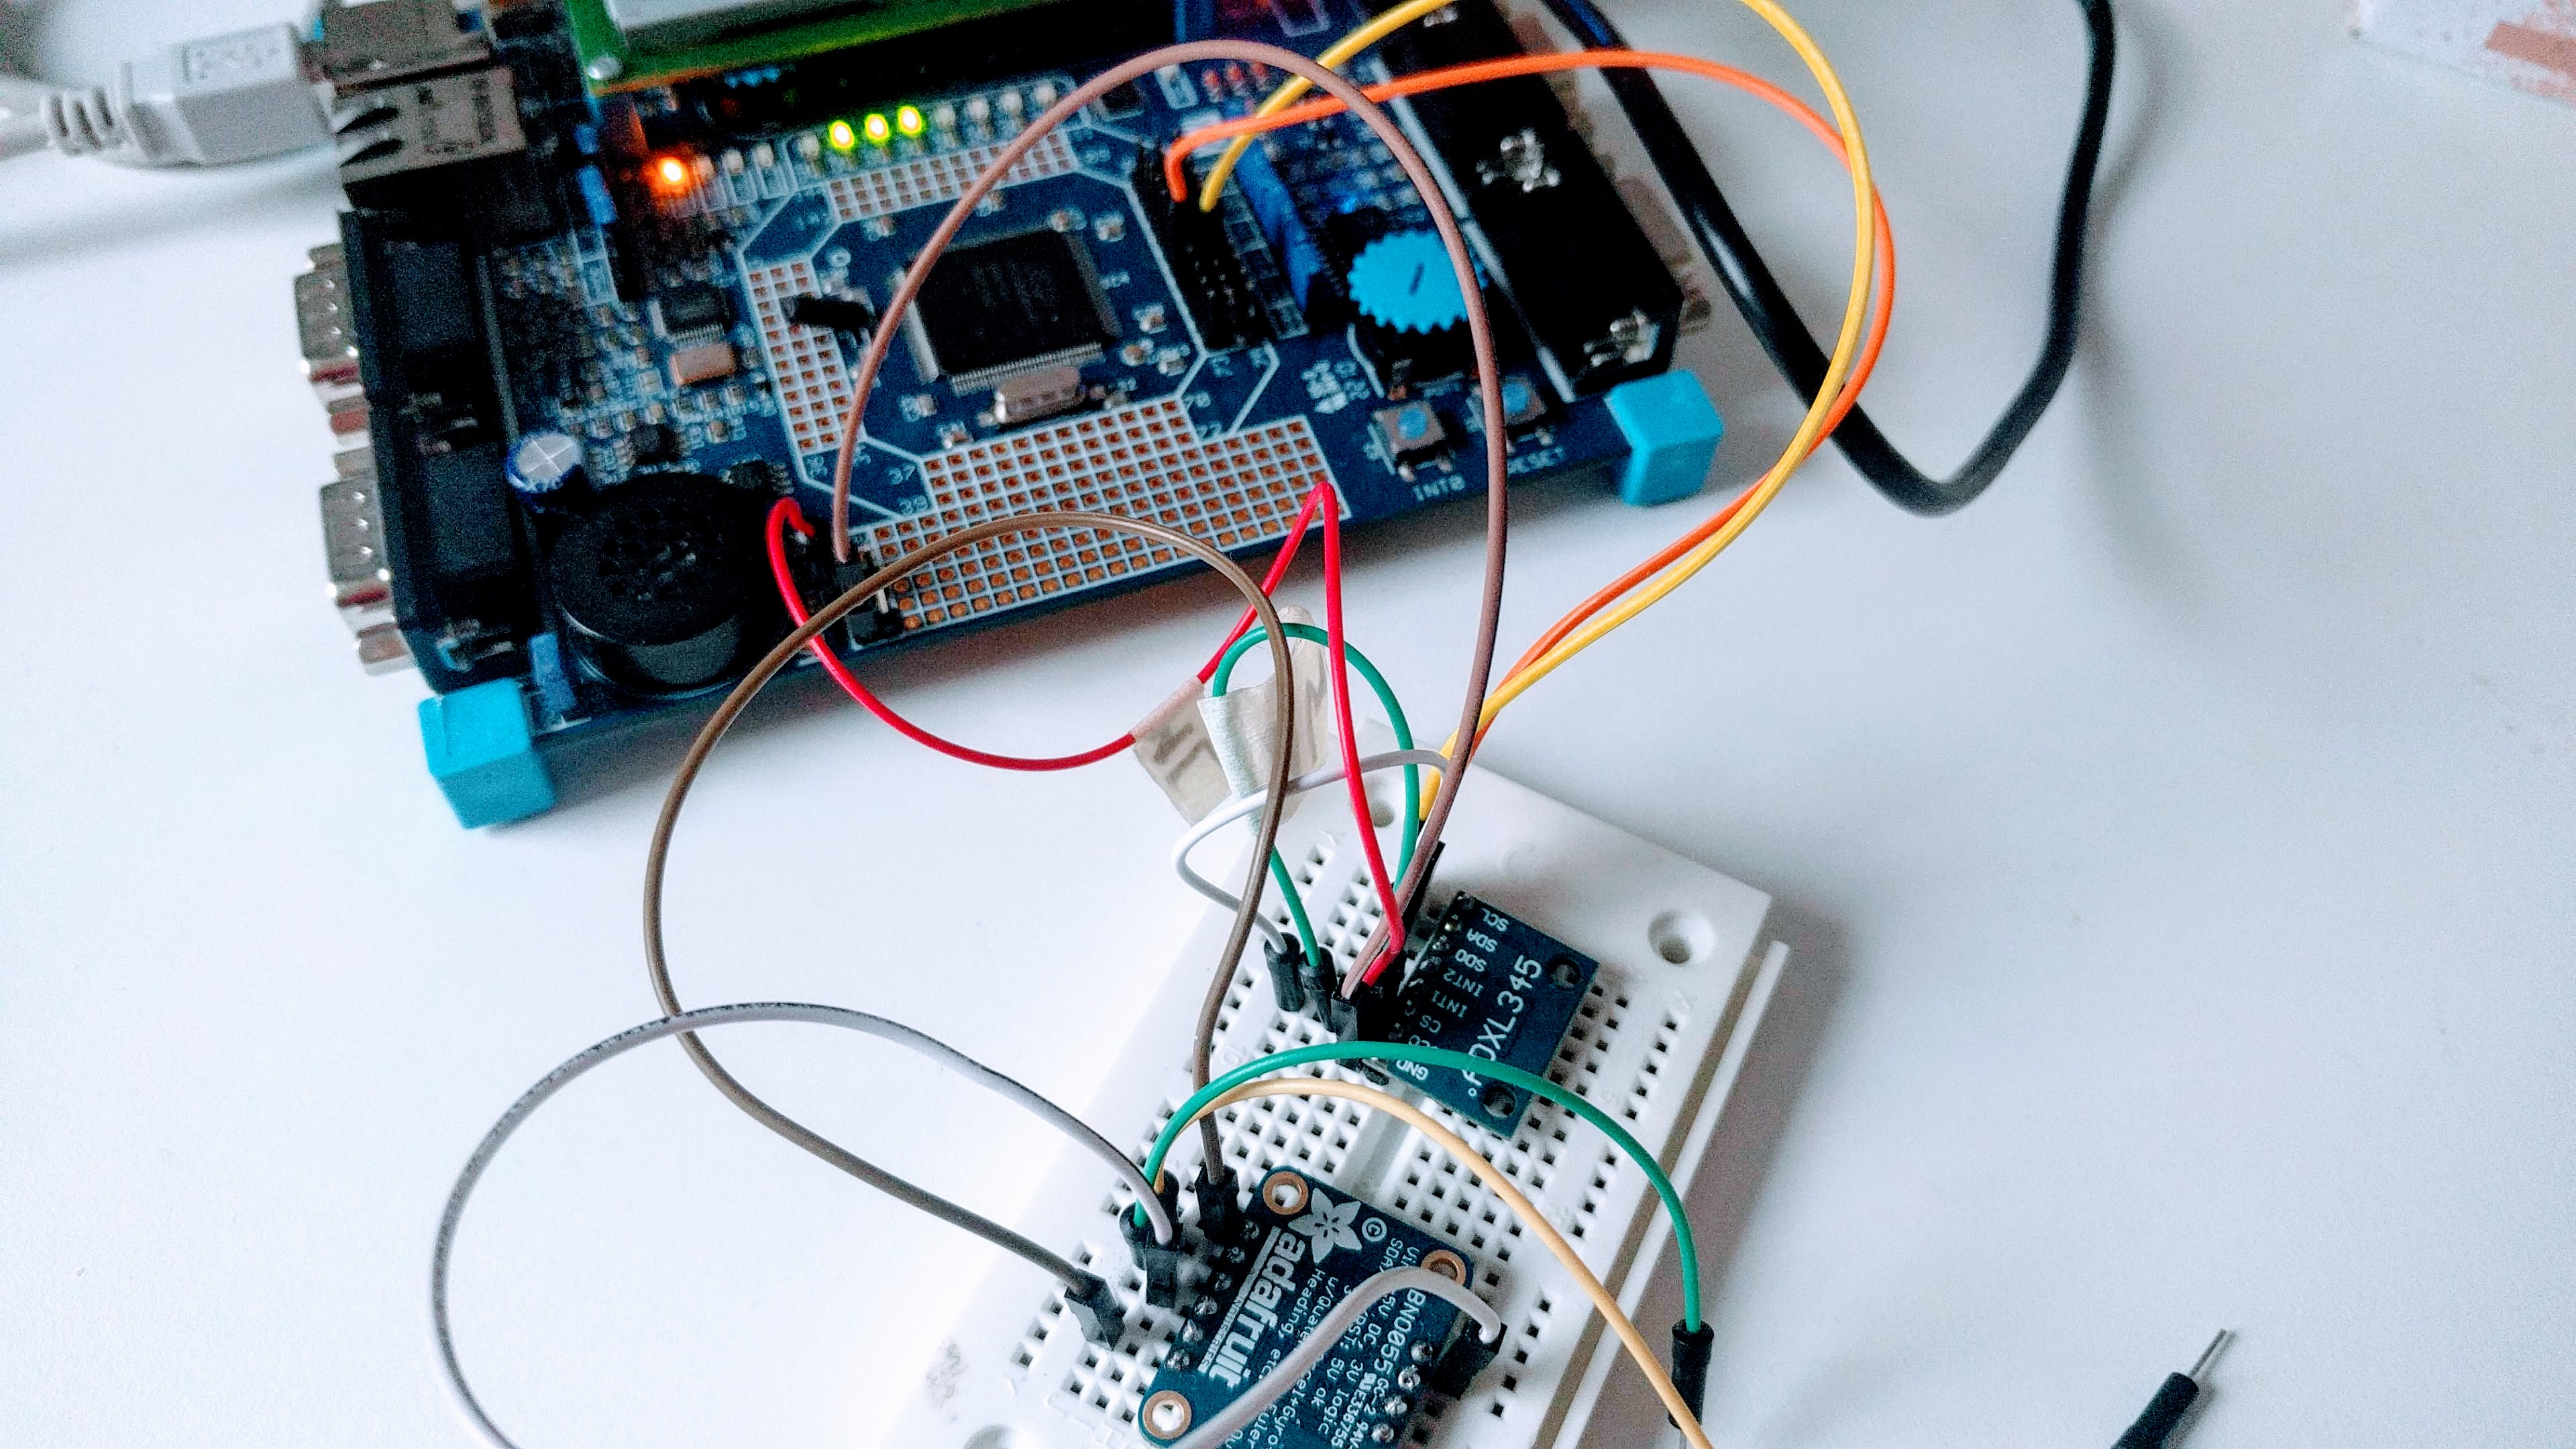
\includegraphics[width=1\linewidth]{adx_wires.jpg}
	\caption[AXL345 Pin Belegung]{ADXL345 Pin Belegung}
	\label{fig:i2cwires}
\end{figure}

Die gemessene Daten werden aus die Register \texttt{0x32} bis Register \texttt{0x37} gelesen. Diese sechs Bytes (Register 0x32 bis Register 0x37) sind jeweils acht Bits und enthalten die Ausgangsdaten für jede Achse. Register \texttt{0x32} und Register \texttt{0x33} enthalten die Ausgangsdaten für die X-Achse, Register \texttt{0x34} und Register \texttt{0x35} die Ausgangsdaten für die Y-Achse und Register 0x36 und Register \texttt{0x37} die Ausgangsdaten für die Z-Achse. 

Die Ausgangsdaten sind zwei Komplemente, mit \texttt{DATAx0} als niedrigstwertigem Byte und DATAx1 als höchstwertigem Byte, wobei X, Y oder Z darstellt. Um die Daten richtig zu lesen, wurde es ein Mehrbyte-Lesen von 2 Register durchgeführt und die Daten aus zwei Lesevorgängen nach dem Lesen als 16-Bit Ausgangsdaten dargestellt. 

\begin{lstlisting}
uint16_t i2c16bit = 0x00;
ReadLenght = 2;
GlobalI2CAddr = addr;
I2CMasterBuffer[0] = regs[0];
I2CMasterBuffer[1] = regs[1];
...
// merge the data from two registers
i2c16bit = i2c16bit | I2CReadBuffer[1]; // [REG0, REG1]: REG1 as MSB
i2c16bit = i2c16bit << 8;

i2c16bit = i2c16bit | I2CReadBuffer[0]; // [REG0, REG1]: REG0 as LSB

\end{lstlisting}

\subsection{I2C: Grundlagen und Realisierung auf dem Keil Board}
Für unseres Projekt haben wir I2C Block auf dem Keil Board in Master-Modus programmiert. Mit Master-Sendermodus werden Daten vom Master (Keil Board) zum Slave (Beschleunigungsmesser) übertragen. So erlaubt uns den Beschleunigungsmesser zu initialisieren. 

Im Master-Empfängermodus werden Daten von einem Slave-Sender empfangen. Nach der Initialisierung des Beschleunigungsmessers wird es immer weiter in diesem Modus gearbeitet, da wir nur ständig die ermittelte Position ablesen wollen. 

Für unseres Projekt haben wir I2C1 Block gewählt. Mithilfe von Schaltbild haben wir festgestellt, welche Pins stehen uns zu Verfügung und sind mit anderen Peripheriefunktionen, die während unseres Projekt notwendig sein könnten, nicht belegt. 

\begin{figure}[!hb]
	\centering
	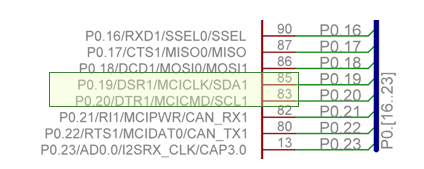
\includegraphics[width=0.6\linewidth]{pins_gyro.jpg}
	\caption[I2C1 Pin Belegung]{2C1 Pin Belegung}
	\label{fig:i2cpins}
	\source{Quelle: \cite{keil.mcb2300}(S. 1)}
\end{figure}

\textbf{START- und STOPP-Bedingungen}. Die I2C-Kommunikation mit diesem Gerät wird initiiert, indem der Master eine START-Bedingung sendet und beendet, indem der Master eine STOP-Bedingung sendet. Ein High-to-Low-Übergang auf der SDA-Leitung, während der SCL-Pegel hoch ist, definiert eine START-Bedingung. Ein Low-to-High-Übergang Die SDA-Leitung definiert die STOP-Bedingung, während der SCL hoch ist. Dies ist mit der folgenden Abbildung\ref{fig:startstop} gezeigt. 

\begin{figure}[!hb]
	\centering
	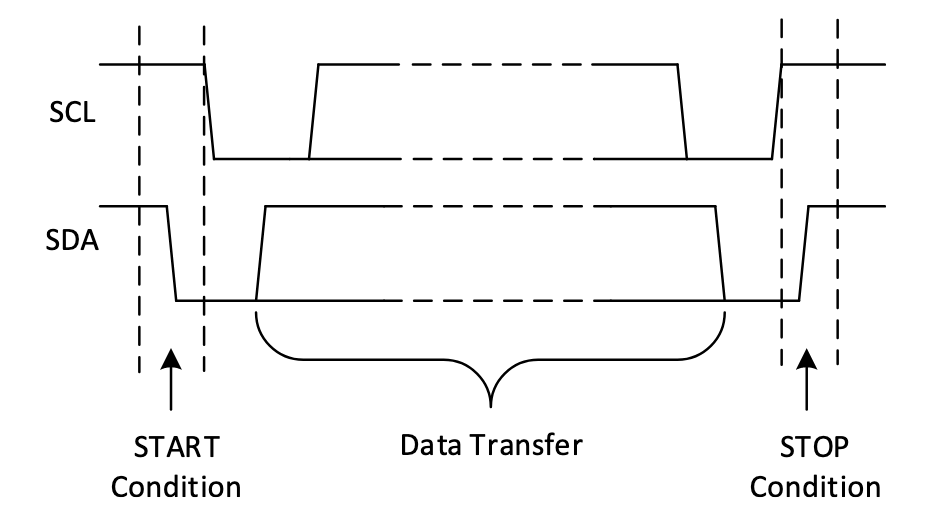
\includegraphics[width=0.6\linewidth]{start_stop.png}
	\caption[I2C Beispiel von START und STOP Bedingungen]{I2C1 Beispiel von START und STOP Bedingungen}
	\label{fig:startstop}
	\source{Quelle: \cite{ti.i2c_bus}(S. 4)}
\end{figure}

Eine \textbf{wiederholte START-Bedingung} sieht ähnlich einer START-Bedingung aus, unterscheidet sich jedoch von einer START-Bedingung, da sie vor einer STOP-Bedingung auftritt (wenn der Bus nicht im Leer ist).

Das \textbf{PCONP}-Register ermöglicht das Deaktivieren ausgewählter Peripheriefunktionen, um Energie zu sparen. Wenn ein Peripheriesteuerbit 1 ist, ist dieses Peripheriegerät aktiviert. Wenn ein Peripherie-Bit 0 ist, wird die Uhr des Peripheriegeräts deaktiviert, um Energie zu sparen. Dem I2C1 entspricht das Bit 19 in PCONP-Register. Um I2C1 zu aktivieren, muss man den Wert $2^{19}$ ins Register schreiben, was in Hexadezimal Format $0x00080000$ entspricht. Mit der Verwendung von logischen Operator $OR$ wird die I2C1 aktiviert und die andere Peripheriefunktionen unverändert geblieben.
\begin{lstlisting}
PCONP |= 0x00080000;
\end{lstlisting}
Die nächste Schritte erlauben es, die Interrupt zu aktivieren. Da dem I2C1 das Bit 19 entspricht, wird es immer mit 19 Bit in jedem Register gearbeitet. \textbf{Vector Address Registers 0-31} (VICVectAddr0-31 sind schreibgeschützte Register. Diese Register enthalten die Adressen der Interrupt-Service-Routinen (ISRs) für die 32 vektorisierten IRQ-Slots.
\begin{lstlisting}
VICVectCntl19 = 0x0000001;   // select a priority slot for interrupt
VICVectAddr19 = (unsigned)i2c_irq; //pass the address of the IRQ
VICIntEnable |= 0x00080000; // enable interrupt
PINSEL1 |= 0x000003C0; //Switch GPIO to I2C pins
\end{lstlisting}

Als nächstes wird ein Auswahl der geeigneten I2C-Datenrate und des Arbeitszyklus durchgeführt. Man muss Werte für die Register \textbf{I2SCLH} und \textbf{I2SCLL} einstellen, um die entsprechende Datenrate und den entsprechenden Arbeitszyklus auszuwählen. I2SCLH definiert die Anzahl der PCLK-Zyklen für die SCL-Hochzeit, I2SCLL definiert die Anzahl der PCLK-Zyklen für die SCL-Niedrigzeit. Dafür wird die folgende Formel benutzt:

\begin{equation}
I^2C_{bitfrequency} =  \frac{F_{PCLK}}{I2SCLH + I2SCLL }
\end{equation}\\

Da es mit der Frequenz von 400KHz gearbeitet wird, wird ins PCONP-Register die entsprechenden Werte geschrieben:
\begin{lstlisting}
I21SCLH = 0xF;
I21SCLL  = 0xF;
\end{lstlisting}

Steuerregister \textbf{I2CONSET} und \textbf{I2CONCLR} enthalten Bits, die zur Steuerung der folgenden I2C-Blockfunktionen verwendet werden: Start und Neustart einer seriellen Übertragung, Beenden einer seriellen Übertragung, Bitrate, Adresserkennung und Bestätigung. Der Inhalt des I2C-Steuerregisters kann als I2CONSET gelesen werden. Beim Schreiben auf I2CONSET werden Bits im I2C-Steuerregister gesetzt, die denen im geschriebenen Wert entsprechen. Umgekehrt löscht das Schreiben in I2CONCLR Bits im I2C-Steuerregister, die denen im geschriebenen Wert entsprechen. Während die Initialisierung wird folgendes in die I2CONSET und I2CONCLR geschrieben: 

\begin{lstlisting}
I21CONCLR = 0x000000FF; // Clear all I2C settings
I21CONSET = 0x00000040; // Enable the I2C interface
\end{lstlisting}

Schieberegister \textbf{I2DAT} enthält ein Byte der zu übertragenden seriellen Daten oder ein gerade empfangenes Byte. Daten in I2DAT werden immer von rechts nach links verschoben. Das erste zu sendende Bit ist das MSB (Bit 7), und nachdem ein Byte empfangen wurde, befindet sich das erste Bit der empfangenen Daten im MSB von I2DAT. 

Der \textbf{Master-Sendermodus} kann jetzt durch Setzen des STA-Bits aufgerufen werden. Die I2C-Logik testet nun den I2C-Bus und generiert eine Startbedingung, sobald der Bus frei wird. Wenn eine START-Bedingung übertragen wird, wird das serielle Interrupt-Flag (SI) gesetzt und der Statuscode im \textbf{Statusregister (I2STAT)} wird 0x08 sein. Dieser Statuscode wird von der Interrupt-Service-Routine verwendet, um die entsprechende Status-Service-Routine einzugeben, die I2DAT mit der Slave-Adresse und dem Datenrichtungsbit (SLA + W) lädt. Die Abbildung \ref{fig:write} zeigt das Schreiben ins Slave's Register.
\begin{figure}[!hb]
	\centering
	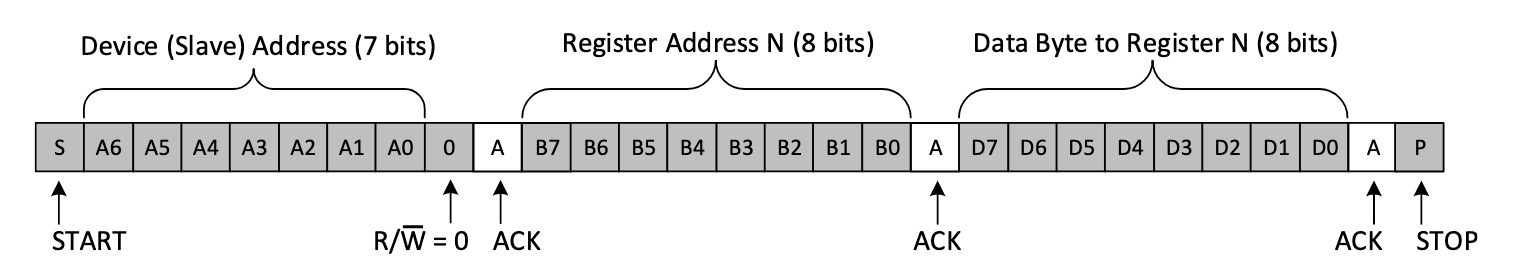
\includegraphics[width=0.8\linewidth]{write.png}
	\caption[I2C Beispiel Schreiben ins Slave Device's Register]{I2C Beispiel Schreiben ins Slave Device's Register}
	\label{fig:write}
	\source{Quelle: \cite{ti.i2c_bus}(S. 7)}
\end{figure}\\
\begin{figure}[!hb]
	\centering
	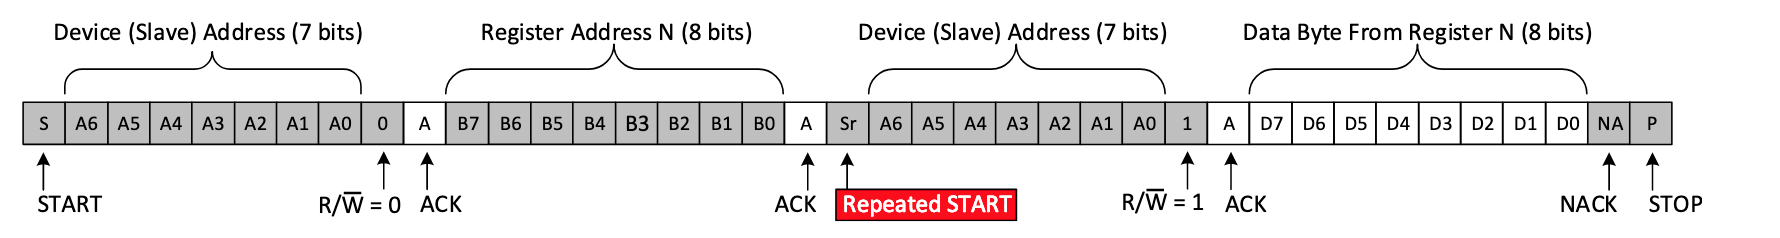
\includegraphics[width=1\linewidth]{read.png}
	\caption[I2C Beispiel Lesen vom Slave Device's Register]{I2C Beispiel Lesen vom Slave Device's Register}
	\label{fig:read}
	\source{Quelle: \cite{ti.i2c_bus}(S. 7)}
\end{figure}\\

Im \textbf{Master-Empfängermodus} werden einige Datenbytes von einem Slave-Sender empfangen. Die Übertragung wird wie im Mastersender-Modus initialisiert. Wenn die Startbedingung übertragen wurde, muss die Interrupt-Service-Routine I2DAT mit der 7-Bit-Slave-Adresse und dem Datenrichtungsbit (SLA + R) laden. Wenn die Slaveadresse und das Datenrichtungsbit gesendet und ein Bestätigungsbit empfangen wurde, wird das serielle Interrupt-Flag (SI) erneut gesetzt und eine Nummer festgelegt Statuscodes in I2STAT sind möglich. Die Abbildung \ref{fig:read} zeigt das Lesen vom Slave's Register.

\subsection{Software}
Die Slave-Adresse und die zu sendenden Daten werden in globalen Variablen abgelegt, damit sie vom I2C Interrupt-Routine verwendet werden können. Die Adresse ist eine Sieben-Bit-Adresse, wobei das LSB zum Schreiben eingestellt und zum Lesen gelöscht ist. Als nächstes löscht die Routine die I2C-Steuerflaggen, aktiviert die I2C-Peripherie und gibt eine Startbedingung aus. Nachdem die Startbedingung auf den Bus geschrieben wurde, wird ein Interrupt generiert, und ein Ergebniscode kann aus dem I2C-Statusregister gelesen werden.

\begin{lstlisting}
unsigned int ADXLI2CAdresss = 0x3A;
unsigned char GlobalI2CAddr;
unsigned char GlobalI2CReg;
unsigned char GlobalI2CData;
unsigned char GlobalI2CRead;
\end{lstlisting}

Wenn die Startbedingung erfolgreich war, lautet der Code im I2STAT-Register 0x08. Als nächstes muss die Anwendungssoftware die Slave-Adresse und das R / W-Bit in das I2Cdata-Register schreiben. Wenn die Bestätigung empfangen wird, wird ein weiterer Interrupt generiert, und das Statusregister I2STAT enthält den Code 0x18, wenn die Übertragung erfolgreich war. Nachdem der Slave nun adressiert wurde und bereit ist, Daten zu empfangen, können wir eine Bytefolge in das I2C-Datenregister schreiben. Wenn jedes Byte geschrieben wird, wird es übertragen und bestätigt. Bei Bestätigung wird ein Interrupt generiert und 0x28 befindet sich im Statusregister, wenn die Übertragung erfolgreich war. Wenn es fehlschlug und ein NACK vorhanden war, lautet der Code 0x20 und das Byte muss erneut gesendet werden. Wenn also jedes Byte übertragen wird, wird ein Interrupt generiert, der Statuscode kann geprüft und das nächste Byte gesendet werden. Nachdem alle Bytes gesendet wurden, kann die Stoppbedingung durch Schreiben in das I2C-Steuerregister aktiviert werden, und die Transaktion ist abgeschlossen. Die Abbildung\ref{fig:master_write} und  Abbildung\ref{fig:master_read} zeigen die Zustände, die im I2STAT-Register eintreten werden.

\begin{figure}[!ht]
	\centering
	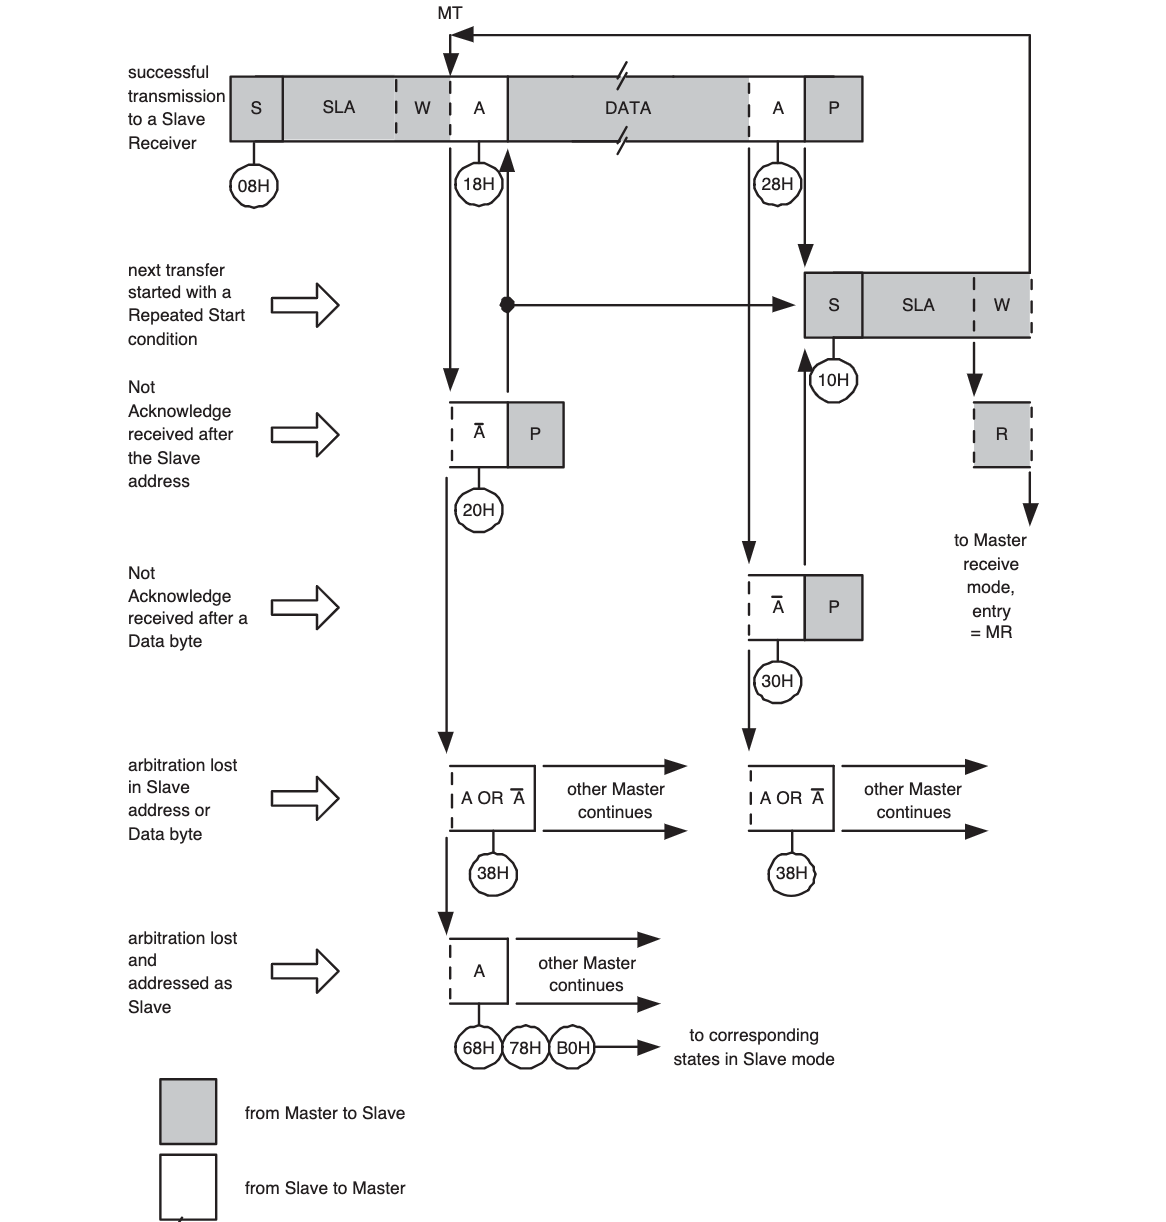
\includegraphics[width=1\linewidth]{master_write.png}
	\caption[I2STAT-Register während Schreiben]{I2C Zustände ins I2STAT-Register während Schreiben}
	\label{fig:master_write}
	\source{Quelle: \cite{nxp.lpc23xx.user_manual}(S. 520)}
\end{figure}
\begin{figure}[!ht]
	\centering
	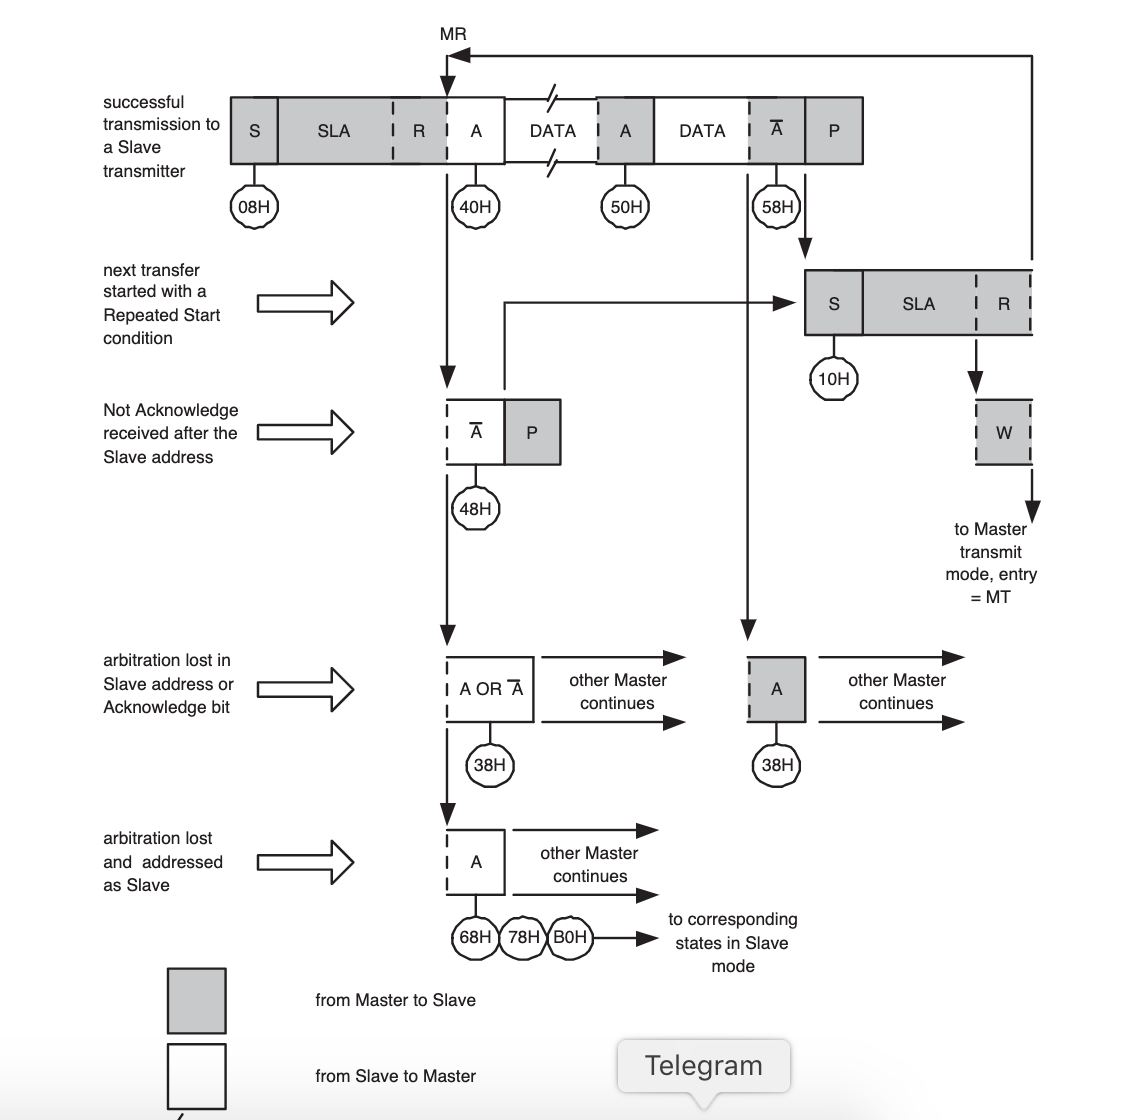
\includegraphics[width=1\linewidth]{master_read.png}
	\caption[I2STAT-Register während Lesen]{I2C Zustände ins I2STAT-Register während Lesen}
	\label{fig:master_read}
	\source{Quelle: \cite{nxp.lpc23xx.user_manual}(S. 521)}
\end{figure}
\clearpage

Um das Lesen des Quellcodes zu vereinfachen, werden die entsprechenden Zuständen als $enum$-type deklariert:
\begin{lstlisting}
volatile enum {
	I2C_IDLE,
	I2C_ADR,
	I2C_STARTED,
	I2C_RESTARTED,
	I2C_REG,
	I2C_DAT,
	I2C_DAT_ACK,
	I2C_RESTART,
	I2C_DAT_NACK,
	I2C_WRITE,
	I2C_READ,
	I2C_ERR,
	I2C_LOST,
	I2C_DONE
} GlobalI2CState;
\end{lstlisting}

Um die gemessene Daten vom dem Beschleunigungsmesser ADXL345 zu lesen, werden die 6  Register verwendet. Die I2C Interrupt Service Routine wird erweitert und damit ein Mehrbyte-Lesen von 2 Register durchgeführt. Die Ausgangsdaten sind zwei Komplemente, mit DATAx0 als niedrigstwertigem Byte und DATAx1 als höchstwertigem Byte, wobei x X, Y oder Z darstellt. 
\begin{lstlisting}
unsigned char XRegs[] = {ADXL345_REG_DATAX0, ADXL345_REG_DATAX1};
unsigned char YRegs[] = {ADXL345_REG_DATAY0, ADXL345_REG_DATAY1};
unsigned char ZRegs[] = {ADXL345_REG_DATAZ0, ADXL345_REG_DATAZ1};
\end{lstlisting}
	
Der I2C-Interrupt ist einfach eine Zustandsmaschine, die das Statusregister für jeden Interrupt untersucht und die erforderliche Aktion ausführt. Dies kann als SWITCH-Anweisung implementiert werden, wie unten es der Teil der Funktion zeigt.
\begin{lstlisting}
__irq void i2c_irq(void) {
	switch (I21STAT) // Read result code and switch to next action
	{
	...
	
	case (0x28): // Data byte in I2DAT  transmitted; ACK  received.
	case (0x30): // transmitted, NOT ACK has been received
		// Repeated Start for Read Operation
		// Case RESTART -> READ
		if (GlobalI2CState == I2C_REG && GlobalI2CRead) {
			I21CONSET = 0x24; // Repeated start condition for Read Access
			I21CONCLR = 0x08; // clear SI flag
			GlobalI2CState = I2C_READ;
		}
		// Case RESTART -> WRITE
		else if (GlobalI2CState == I2C_REG && !GlobalI2CRead) {
			// with re-start for write
			//I21CONSET = 0x24; // Repeated start condition for Write Access
			//I21CONCLR = 0x08; // clear SI flag
			GlobalI2CState = I2C_WRITE;
		}
		
		if (GlobalI2CState == I2C_WRITE) {
			I21DAT = GlobalI2CData;
			GlobalI2CState = I2C_DAT;
			I21CONCLR = 0x08; // clear SI flag
		}
		else if (GlobalI2CState == I2C_DAT) {
			GlobalI2CState = I2C_DONE;
			I21CONSET = 0x10; // STO
			I21CONCLR = 0x08; // clear SI flag
		}
		break;
	....
	
	/* Data has been received, ACK returned. Data read from I2DAT.
	Additional data will be received. If this is the last data byte 
	then NOT ACK will be returned,
	otherwise ACK will be returned */
	case (0x50):
	case (0x58): // Data Received, Not Ack
		if (ReadIndex != ReadLenght) {
			GlobalI2CData = I21DAT;
			I2CReadBuffer[ReadIndex] = I21DAT;
			ReadIndex++;
			I21CONCLR = 0x0C; //clear the SI flag and the AA bit
			GlobalI2CState = I2C_DAT_ACK;
		}
		else {
			ReadIndex = 0;
			I21CONSET = 0x10; // set STO
			GlobalI2CState = I2C_DONE;
		}
		I21CONCLR = 0x08; // clear SI flag
		break;
	
	default:
		break;
	}	
	VICVectAddr = 0x00000000; // Clear interrupt in
}
\end{lstlisting}

Das Schreiben wird vom Lesen mithilfe des Flags $GlobalI2CRead$ unterscheidet. Wird $GlobalI2CRead$ von Software auf 1 gesetzt, wird dann die wiederholte START-Bedingung erzeugt und I2C-Interrupt wird mit dem Zustand $0x10$ gesetzt und das Lesen wird durchgeführt. 

\begin{lstlisting}
void I2CWriteReg(unsigned char addr, unsigned char reg, 
unsigned char data) {
	...
	GlobalI2CData = data;
	GlobalI2CRead = 0;
	GlobalI2CState = I2C_ADR;
	I21CONSET = 0x20; // Start condition
}
\end{lstlisting}

\begin{lstlisting}
uint16_t I2CRead16Bits(unsigned char addr, unsigned char regs[])  
{
	...
	GlobalI2CRead = 1;
	GlobalI2CState = I2C_ADR;
	I21CONSET = 0x20; // Start condition
}
\end{lstlisting}

Es wird im I2C Zustand $0x28$ unterscheidet, ob es Lesen oder Schreiben durchführen werden sollen.
\begin{lstlisting}
if (GlobalI2CState == I2C_REG && GlobalI2CRead) {
     // Case RESTART -> READ
	I21CONSET = 0x24; // Repeated start condition for Read Access
	I21CONCLR = 0x08; // clear SI flag
	GlobalI2CState = I2C_READ;
}
// Case RESTART -> WRITE
else if (GlobalI2CState == I2C_REG && !GlobalI2CRead) {
	//I21CONCLR = 0x08; // clear SI flag
	GlobalI2CState = I2C_WRITE;
\end{lstlisting}

Nach dem wiederholten Start-Bedingung wird es nach dem Zustand $0x10$ gewechselt und dann den Flag für Lesen auf 1 gesetzt:
\begin{lstlisting}
if(GlobalI2CState == I2C_READ) {
	// Write Slave Address with R/W bit to I2DAT
	I21DAT = GlobalI2CAddr | 1; // Send address and read bit R/W = 1
}
\end{lstlisting}

Nach der Implementierung alle oben genannten Verfahren, werden die gemessene Daten vom digitalen Beschleunigungsmesser ADXL345 angelesen. Die abgelesene Daten können weiter in Programm verwendet werden und die Position von Komponenten der LED-Panels ansteuern.


\clearpage
\label{chap:impl:ledcube}
%Beschreibung der Implementierung der Darstellungen auf den Displays
Die Komponente LED-Panels empfängt Daten der Panelinformationen von der Komponente Flüssigkeitssimulation und beleuchtet die Panels entsprechend dieser Daten. Die Anzahl der Wasserteilchen pro Pixel dient als Intensität der blauen Farbe.

\subsection{Hardware}
Der RGB-Würfel wird aus sechs 32$\times$32 RGB Matrix LED-Panels aufgebaut. Betrieb eines Panels benötigt den Strom von ungefähr $2A$. Die 6 Panels werden anhand einer Stromversorgung geschaltet. Auf der Rückseite des Panels befinden sich ein Eingangs- und ein Ausgangsport mit jeweils 16 Pins. Diese sind für die Farbinformation R1, G1, B1, R2, G2, B2, die Adresssignale A, B, C, D und die Steuersignale CLK (Takt), OE (Output Enable), LAT (Latch), und 3 GNDs. Ein Panel wird somit über 16 Kabel direkt mit dem Board verbunden (Abbildung \ref{fig:led:plug}) und die restlichen fünf Panels werden nebeneinander anhand Flachbandkabel verbunden, welches Daisy-Chain genannt wird (Abbildung \ref{fig:led:chain}). 

\begin{figure}
	\centering
	\begin{minipage}[t]{0.45\linewidth}
	\includegraphics[width=.9\linewidth]{example-image-a}
	\caption{Daten- und Steuersignale mit Beschriftung von Buchse bzw. Flachbandkabel}
	\label{fig:led:plug}
	\end{minipage}
	\hspace{0.05\linewidth}
	\begin{minipage}[t]{0.45\linewidth}
	\includegraphics[width=.9\linewidth]{example-image-b}
	\caption{Panels per Daisy-Chain}
	\label{fig:led:chain}
	\end{minipage}
\end{figure}

Die Eingänge der RGB-, Adress- und Steuersignale eines Panels werden mit GPIO (General Purpose Input Output) Pins auf dem Board verbunden, Port 2.0 bis 2.5 bzw. Port 3.0 bis 3.6. Als Default-Einstellung vom Hersteller sind Port 2.0 bis 2.7 direkt mit den LEDs vom Board verbunden. Daher muss der Jumber XX entnommen werden, um diese Pins für die Anzeige anzuwenden. Abbildung \ref{fig:assembly:dice} stellt den gesamten Aufbau der Komponente Würfel dar.
\begin{figure}
	\centering
	\includegraphics[width=0.95\linewidth]{example-image}
	\caption[Aufbau von sechs 32$\times$32 RGB Matrix LED-Panels]{Aufbau von sechs 32$\times$32 RGB Matrix LED-Panels. }
	\label{fig:assembly:dice}
\end{figure}

\subsection{Konfiguration und Mechanismus einer Anzeige}
Hier wird beschrieben, wie ein aus 32 Zeilen $\times$ 32 Spalten insgesamt 1024 LEDs bestehendes Panel gesteuert wird. Die  RGB-Signale R1, G1 und B1 sowie R2, G2 und B2 enthalten die Farbinformationen eines Pixels des oberen bzw. unteren Teil des Panels. Das Panel installiert 32-bit Schieberegister, womit die kompletten Farbdaten einer Zeile gespeichert werden. Das Verschieben geschieht durch das Taktsignal. Es lässt somit zwei Zeilen gleichzeitig anzeigen. Dies soll in schneller als 20 $ms$ geschehen, damit menschliche Augen einen Anzeigewechsel nicht merken und diesen als ein Standbild erfassen. Diese zwei Zeilen sind erste und 17. Zeile, zweite und 18. Zeile, ..., und 16. und 32. Zeile, die jeweils durch eine Adresse festgelegt werden, welche von den Adresssignale A, B, C und D definiert wird.\\

\emph{<Schritte>}
\begin{enumerate}
	\item Setzen alle Pins auf \texttt{Low} (anfang)
	\item \texttt{R1,G1,B1,R2,G2,B2} Pins auf \texttt{High/Low} setzen
	\item \texttt{CLK} Pin auf \texttt{High} setzen
	\item \texttt{CLK} Pin auf \texttt{Low} setzen \\
	(Farbinformation wird in den Schiebregister geladen.)
	\item Schritte 2-4 für alle Spalten wiederholen
	\item Mit Adresspins \texttt{ABCD} eine gezielte Zeile (von der oberen und unteren Hälfte) auswählen
	\item \texttt{OE} Pin auf \texttt{High} setzen
	\item \texttt{LAT} Pin auf \texttt{High} setzen (erleuchtet LED)
	\item \texttt{LAT} Pin auf \texttt{Low} setzen
	\item \texttt{OE} Pin auf \texttt{Low} setzen
	\item Zurück zum Schritt 1
\end{enumerate}

Werden Panels verkettet, werden die Signale seriell weiter geleitet und die Farbinformation muss daher bis zum letzten Spalten reingeschoben werden. Das bedeutet, die verketteten Panels können letztendlich als ein langes Panel betrachtet werden.

Als nächstes soll die Darstellung der Farbintensität betrachtet werden. Das Display besitzt keine PWM-Funktionalität und lässt ein LED nur \texttt{An} oder \texttt{Aus} schalten. Um unterschiedliche Blaufarben zu realisieren, wird die Methode von Binary Code Manipulation verwendet (siehe XXX zum Detail). 

\subsection{Software}
 Zur Anwendung GPIO Pins müssen die folgenden Schritte (Quelltext \ref{code:ledinit}) durchgeführt werden.
\begin{lstlisting}[language={c}, caption={Initialisierung von GPIO als Output}, label={code:ledinit}]
void led_init(void)
{
    PINSEL10 = 0;    ///< Disable ETM interface, enable LEDs (turn all LEDs on)
    PINSEL4 = 0;     ///< Set function GPIO on port 2
    FIO2DIR  = 0xFF; ///< P2.0..7 defined as output
    FIO2MASK = 0;    ///< Enable write, set, clear, and read to R/W port 2
}

void led32x32_init(void)
{
    led_init();

    // Set port 3
    PINSEL6 = 0;     ///< Set function GPIO on port 3.0..5
    FIO3DIR = 0xFF;  ///< P3.0..7 defined as output
    FIO3MASK = 0;    ///< Enable write, set, clear, and read to R/W port 3
}
\end{lstlisting}

Zur Steuerung der Signale werden die Unterfunktionen (Quelltext \ref{code:ctrlsig}) geschrieben. Durch \texttt{FIO2SET} und \texttt{FIO2CLR} Register (analog zu \texttt{FIO3}) wird der Ausgang eines Pins auf \texttt{1} bzw. auf \texttt{0} gesetzt. Diese Grundfunktionen werden in den jeweiligen Funktionen (RGB-Signale, Adresssignale und Steuersignale) aufgerufen.

\begin{lstlisting}[language={c}, caption={Funktionen zur Steuerung der Signale.}, label={code:ctrlsig}]
#define LED32X32_RGBPIN_SETTER   FIO2SET
#define LED32X32_RGBPIN_CLEANER  FIO2CLR
#define LED32X32_CTRLPIN_SETTER  FIO3SET
#define LED32X32_CTRLPIN_CLEANER FIO3CLR

static inline void lp32x32_setCtrlPin(int pin)
{
    LED32X32_CTRLPIN_SETTER |= (1 << pin);
}
static inline void lp32x32_clearCtrlPin(int pin)
{
    LED32X32_CTRLPIN_CLEANER |= (1 << pin);
}
static inline void lp32x32_setRgbPin(int pin)
{
    LED32X32_RGBPIN_SETTER |= (1 << pin);
}
static inline void lp32x32_clearRgbPin(int pin)
{
    LED32X32_RGBPIN_CLEANER |= (1 << pin);
}
\end{lstlisting}

Überlagerung mehreren Schichten zur Realisierung einer 24-bit Farbe wird dadurch implementiert, dass der Zyklus der 1-zeiligen Anzeige entsprechend wiederholt wird. Dazu benötigt das System noch einen schnelleren Takt. Quelltext \ref{code:ledmain} zeigt die Hauptfunktion des Moduls LED32x32.

\begin{lstlisting}[language={c}, caption={Schritte von Panel-Anzeige}, label={code:ledmain}]

void lp32x32_refresh_chain_24bit_rgb(panel_t panels[CHAIN_LEN])
{
    static uint8_t row = 0;
    static uint8_t color_bit = 0;
    uint8_t col;
    uint8_t layer;
    uint8_t panelIndex = 0;
    uint32_t upperPixel = 0;
    uint32_t bottomPixel = 0;

    for(layer = 0; layer < 1; ++layer)
    {
        for(col = 0; col < (COL_NUM * CHAIN_LEN); ++col)
        {
            panelIndex = col / COL_NUM;
            upperPixel = panels[panelIndex][row][col - COL_NUM * panelIndex].particle_count;
            bottomPixel = panels[panelIndex][row + ROW_NUM / 2][col - COL_NUM * panelIndex].particle_count;
            
            lp32x32_setUpperPixelInfo((/*red=  */((upperPixel  & LED32X32_RGB24_R_MASK) >> 16) & (0x01 << color_bit)), 
                                       (/*green=*/((upperPixel  & LED32X32_RGB24_G_MASK) >>  8) & (0x01 << color_bit)),
                                       (/*blue= */((upperPixel  & LED32X32_RGB24_B_MASK)      ) & (0x01 << color_bit)));
            lp32x32_setBottomPixelInfo((/*red=  */((bottomPixel & LED32X32_RGB24_R_MASK) >> 16) & (0x01 << color_bit)), 
                                       (/*green=*/((bottomPixel & LED32X32_RGB24_G_MASK) >>  8) & (0x01 << color_bit)),
                                       (/*blue= */((bottomPixel & LED32X32_RGB24_B_MASK)      ) & (0x01 << color_bit)));

            lp32x32_clock(); ///< Shift RGB information of each pixel to horizontal direction
        }

        lp32x32_setRow(row);
        lp32x32_setCtrlPin(LED32X32_PIN_OE);
        lp32x32_latch();
        lp32x32_clearCtrlPin(LED32X32_PIN_OE);
    }
    ++row;
    if(row >= (ROW_NUM/2))
    {
        row = 0;
        ++color_bit;
    }
    if(color_bit >= 8)
    {
        color_bit = 0;
    }
}
\end{lstlisting}

\clearpage

\chapter{Ergebnis}


\clearpage




%%%%%%%%%%%%%%%%%%%%%%%%%%%%%%%%%%%%%%%%%%%%%%%%%%%%%%%%%%%%%%%
%% Literaturverzeichnis
\clearpage\newpage
\addcontentsline{toc}{chapter}{Literatur- und Quellenverzeichnis}
\bibliography{bhtThesis.bib}

\end{document}
